\documentclass{article}
\usepackage[utf8]{inputenc}
\usepackage{algorithmic, amsmath, amsthm, amsfonts, amssymb,commath, enumerate, tikz, tikz-cd, color, mathrsfs,graphicx}
\graphicspath{ {/Users/David/Desktop/LATEX/HopkinsTalk} }
%tikz is for drawing lattices %tikz-cd is for commutative diagrams
															%color is for making notes in red 
															%mathrsfs is for power set font
%\usepackage[mathscr]{eucal} %mathscr gives nice script fonts

\newtheoremstyle{problemstyle}  % <name> This is my problemstyle. use begin{problem}.
        {12pt}                                               % <space above>
        {}                                               % <space below>
        {}                               % <body font>
        {}                                                  % <indent amount}
        {\bfseries}                 % <theorem head font>
        {\normalfont\bfseries.}         % <punctuation after theorem head>
        {.5em}                                          % <space after theorem head>
        {}                                                  % <theorem head spec (can be left empty, meaning `normal')>


\theoremstyle{problemstyle}

\newtheorem{problem}{Problem}

\theoremstyle{problemstyle}

\newtheorem{definition}{Definition}

\theoremstyle{problemstyle}

\newtheorem{example}{Example}

\theoremstyle{problemstyle}

\newtheorem{lemma}{Lemma}

\theoremstyle{problemstyle}

\newtheorem{proposition}{Proposition}

\theoremstyle{problemstyle}

\newtheorem{solution}{Solution}

\theoremstyle{problemstyle}

\newtheorem{theorem}{Theorem}

\theoremstyle{problemstyle}

\newtheorem{exercise}{Exercise}

\tikzcdset{every label/.append style = {font = \small}}

\tikzset{%
    symbol/.style={%
        draw=none,
        every to/.append style={%
            edge node={node [sloped, allow upside down, auto=false]{$#1$}}}
    }
}

\title{ \vspace{-10ex} %uncomment to remove vertical space
%title of assignment goes here e.g. "Math 721 Homework 3"
Johns Hopkins Category Theory Seminar\\ 
tslil clingman\\ 
What is an LCC?
}

\author{David L. Meretzky
}


\date{%date assignment is due goes here
Thursday November 9th, 2018
} 


\renewcommand*{\thefootnote}{$\dagger$} %changes default footnote marking to a dagger instead of a number (numbers are sometimes mistaken for citations)

\begin{document}

\maketitle


\subsection{What is an LCC?}

\begin{definition}
A cartesian closed category is a category $\mathcal{C}$ in which all finite products exist and the product functor has a right adjoint. 
\end{definition}

Note that the empty product in a category is a terminal object. The empty product is the limit over the empty diagram. Thus any cartesian closed category has a terminal object. The statement that the product functor has a right adjoint means that it has exponential objects. This says in fancier language that it is closed with respect to it's cartesian monoidal structure.\footnote{A cartesian monoidal category is a monoidal category whose monoidal structure is given by the category theoretic product. Closure means that the hom-sets are internal.}\\

%Group is not CCC because it does not have exponentials. There is no natural way to enrich the hom sets of Group over itself. The category of abelian groups is another matter.  This disagrees with the chart below.  \\ 

%\text{CAT} the category of \textit{small} categories is CCC because we can show that \text{CAT} has finite products.  This follows from the fact that $SET$ has finite products. See exercise *** of Leinster. We then need to show that \text{CAT} has an internal hom which is a right adjoint to the product functor.\\ 

%We need to show that for any small categories $\mathcal{C}$ and $\mathcal{D}$, the functor category $[\mathcal{C},\mathcal{D}]$ is a small category. 

\begin{definition}
A locally cartesian closed category is a category $\mathcal{C}$ together with a functor $\mathcal{C}/(-):\mathcal{C}^{op} \rightarrow \text{CAT}$.
On objects $A$ of $\mathcal{C}^{op}$, $\mathcal{C}/A$ is the slice category over $A$. On morphisms $C' \xrightarrow[]{c} C$, $\mathcal{C}/c$ is a functor of slice categories. Let $c^* = \mathcal{C}/c:\mathcal{C}/C \rightarrow \mathcal{C}/C'$ defined on objects by the left vertical leg of the pullback square: 

\begin{center}
\begin{tikzcd}
c^*X \arrow[r] \arrow[d,"c^*f"'] & X \arrow[d,"f"]  \\
C'  \arrow[r,"c"'] & C 
\end{tikzcd}
\end{center}

Furthermore, $\mathcal{C}/(-)$ has a right adjoint denoted $\Pi_{(-)}$. 
\end{definition}

We are going to investigate the adjunction: 

\begin{center}
\begin{tikzcd}
\text{CAT} \ar[d, bend left,"","\Pi_{(-)}"{name=A, right}]  \\
\mathcal{C}^{op} \ar[u, bend left,"","\mathcal{C}/(-)"{name=B, left}] \ar[from=B, to=A, symbol=\dashv]
\end{tikzcd}
\end{center}

\begin{example}
What is the relationship between locally cartesian closed and cartesian closed?\\
\begin{center}
\begin{tabular}{|l|l|l|}
\hline
Category & LCC  & CC \\ \hline
SET & \checkmark  & \checkmark \\ \hline
CAT & $\times$ & \checkmark \\ \hline
GRP & $\times$ & \checkmark \\ \hline
Top & $?$ & $?$ \\ \hline
Topos & \checkmark & \checkmark \\ \hline
\end{tabular}
\end{center}
\end{example}

\begin{exercise}\footnote{tslil comments that this holds in any category $\mathcal{C}$ which has pullbacks.}
Given the diagram $B \xrightarrow[]{f} A$ in $\mathcal{C}$, show that the left adjoint to $f^*:\mathcal{C}/A \rightarrow \mathcal{C}/B$ is the functor $\Sigma_f(\begin{tikzcd}[cramped, sep=small] X \arrow[rd, "b", start anchor={[xshift=-.6ex, yshift= .7ex]},end anchor={[xshift=.7ex, yshift= -.7ex]}]  &  \\  &  B \end{tikzcd}) = \begin{tikzcd}[cramped, sep=small] X \arrow[rd, "f\circ b", start anchor={[xshift=-.6ex, yshift= .7ex]},end anchor={[xshift=.7ex, yshift= -.7ex]}]  &  \\  &  A \end{tikzcd}$.
\end{exercise}

\begin{solution}
Since slice categories are the order of the day, what better way to prove that this is an adjunction than to show that $f^*\Sigma_f(\begin{tikzcd}[cramped, sep=small] X \arrow[rd, "b", start anchor={[xshift=-.6ex, yshift= .7ex]},end anchor={[xshift=.7ex, yshift= -.7ex]}]  &  \\  &  B \end{tikzcd})/f^*(\mathcal{C}/A)$ is an initial object of $(\begin{tikzcd}[cramped, sep=small] X \arrow[rd, "b", start anchor={[xshift=-.6ex, yshift= .7ex]},end anchor={[xshift=.7ex, yshift= -.7ex]}]  &  \\  &  B \end{tikzcd})/f^*(\mathcal{C}/A)$. Said another way: for any object $\begin{tikzcd}[cramped, sep=small] Y \arrow[rd, "i", start anchor={[xshift=-.6ex, yshift= .7ex]},end anchor={[xshift=.7ex, yshift= -.7ex]}]  &  \\  &  A \end{tikzcd} \in \mathcal{C}/A$ and map $h$, there exist maps $\eta_X$ and $k$ such that the whole diagram commutes. 

\begin{center}
\begin{tikzcd}[sep =large]
X \arrow[rd,"b"'] \arrow[r, "\eta_X", pos = .7] \arrow[rr, "h", bend left] &  f^*\Sigma_f X \arrow[d,"f^*\Sigma_fb", pos=.3] \arrow[r, "k"] & f^*y \arrow[dl,"f^*i"]  \\
& B & 
\end{tikzcd}
\end{center}

The map $\eta_X$ exists because the identity map $id_X$ makes the following diagram commute: 

\begin{center}
\begin{tikzcd}
X \arrow[r,"id_X"] \arrow[d,"b"'] & \Sigma_fX = X  \arrow[d,"\Sigma_fb"]  \\
B  \arrow[r,"f"'] & A 
\end{tikzcd}
\end{center}

Therefore we obtain the morphism $\eta_X$ from the definition of a pullback where we are pulling $\Sigma_fb$ back along $f$. 
\begin{center}
\begin{tikzcd}
X
\arrow[drr, bend left, "id_X"]
\arrow[ddr, bend right, "b"]
\arrow[dr, "\eta_X"] & & \\
& f^*\Sigma_f X \arrow[r] \arrow[d, "f^*\Sigma_fb"]
& \Sigma_fX \arrow[d, "\Sigma_fb"] \\
& B \arrow[r, "f"']
& A
\end{tikzcd}
\end{center}

Now to show that the morphism $k$ exists we note that since $f^*Y$ is defined in terms of a pullback we can form the following commuting diagram:

\begin{center}
\begin{tikzcd}
X \arrow[r,"h"] \arrow[rd, "g"']& f^*Y \arrow[r, "l"] \arrow[d, "f^*i"] & y \arrow[d, "i"] \\
 & B \arrow[r,"f"] & A
\end{tikzcd}
\end{center}

Since $i \circ l \circ h = f \circ g$, we obtain the diagram where we pull back on 

\begin{center}
\begin{tikzcd}
f^*\Sigma_fX \arrow[r,"l'"] \arrow[d, "f^*\Sigma_fg"'] &\Sigma_fX \arrow[r, "l\circ h"] \arrow[d,"\Sigma_fg"'] & Y \arrow[dl,"i"] \\
 B \arrow[r,"f"] &A &
\end{tikzcd}
\end{center}

Since the diagram commutes, we obtain a pullback arrow to $f^*Y$. This completes the verification. 
\end{solution}

tslil calls the following Fruitful Coincidence Number 1: 

\begin{exercise}
With cannonically chosen pullbacks show the natural isomorphism of functors $$[(-)^{op}, SET] \cong SET/(-)$$ from $SET^{op} \rightarrow \text{CAT}$.  
\end{exercise}

\begin{solution}
We need to show that on an object $A$ of $SET$, there is an equivalence of small categories between $[A^{op}, SET]$ and $SET/A$. Furthermore we need to show that this equivalence is natural in $A$. 
For any object $A$ of $SET$, define functors $F_A$ and $G_A$ as follows: 

\begin{center}
\begin{tikzcd}
{[A^{op},SET]} \ar[d, bend left,"","F_A"{name=A, right}]  \\
SET/A \ar[u, bend left,"","G_A"{name=B, left}] \ar[from=B, to=A, symbol=\dashv]
\end{tikzcd}
\end{center}

Let $X,Y \in SET$ and $g:X \rightarrow Y$. Denote a functor from $A$ to $X$ in $[A^{op},SET]$ by just $\{X_a\}_{a \in A}$, an $A$ indexed set. Similarly, we abuse notation to let $g$ mean the morphism in this category which is a natural transformation from $X$ to $Y$, a cofiber-wise mapping. In $SET/A$ we have $g_*:Y/A \rightarrow X/A$ by precomposing the morphism from $Y$ to $A$ with $g$.\\ 

Thinking of functors from $A$ to $X$ in this way, we use the following fact to construct the functor $F_A$: note that in the category of sets, the coproduct of a set $X$ over an indexing set $B$ is exactly the product $B \times X$.  That is, $\Sigma_{b\in B}X = B \times X$.\\

Define $F_A$ by taking the disjoint union, that is the coproduct of $\{X_a\}_{a \in A}$. Thus $F_A(\{X_a\}_{a \in A}) = \Sigma_{a \in A}X_a$. In the case where every $a\in A$ goes to the same set $X$, we have $\Sigma_{a \in A}X_a = A \times X$. This is not true for every functor $X\in[A,SET]$. In the special case we couple this product with the usual projection map we obtain a map over $A$, $\pi_1:A \times X \rightarrow A$. Otherwise, define the map over $A$ to be the map $\pi:\Sigma_{a \in A}X_a\rightarrow A$ by $\pi(X_a) = \pi(X,a) = a$.\\ 

Define $G_A$ which takes in a map over $A$, \begin{tikzcd}[cramped, sep=small] X \arrow[rd, "p", start anchor={[xshift=-.6ex, yshift= .7ex]},end anchor={[xshift=.7ex, yshift= -.7ex]}]  &  \\  &  A \end{tikzcd} and returns an $A$ indexed set $\{X_a\}_{a \in A}$. 

Do this by defining $G_A(\begin{tikzcd}[cramped, sep=small] X \arrow[rd, "p", start anchor={[xshift=-.6ex, yshift= .7ex]},end anchor={[xshift=.7ex, yshift= -.7ex]}]  &  \\  &  A \end{tikzcd}) = \{X_a\}_{a \in A}$ where $X_a = p^{-1}(a)$, the preimage under $p$ of all $a \in A$.\\ 

Firstly we see that the counit of the equivalence is equality.  We have 

\begin{equation}G_{F_A(A)}F_A(\{X_a\}_{a \in A}) = \{X_a\}_{a \in A}\end{equation} in the functor category. 

The unit is also equality. This map, going between \begin{tikzcd}[cramped, sep=small] X \arrow[rd, "p", start anchor={[xshift=-.6ex, yshift= .7ex]},end anchor={[xshift=.7ex, yshift= -.7ex]}]  &  \\  &  A \end{tikzcd} and 
$$F_{G_A(A)}G_A(\begin{tikzcd}[cramped, sep=small] X \arrow[rd, "p", start anchor={[xshift=-.6ex, yshift= .7ex]},end anchor={[xshift=.7ex, yshift= -.7ex]}]  &  \\  &  A \end{tikzcd}) =  \begin{tikzcd}[cramped, sep=small] \Sigma_{a \in A}p^{-1}(a) \arrow[rd, "\pi", start anchor={[xshift=-.6ex, yshift= .7ex]},end anchor={[xshift=.7ex, yshift= -.7ex]}]  &  \\  &  A \end{tikzcd} =  \begin{tikzcd}[cramped, sep=small] \Sigma_{a \in A}X_a \arrow[rd, "\pi", start anchor={[xshift=-.6ex, yshift= .7ex]},end anchor={[xshift=.7ex, yshift= -.7ex]}]  &  \\  &  A \end{tikzcd}$$ is slightly harder to see.\\ 

Firstly, $p$ is defined for all of $X$. Secondly each pair of sets $X_a$ and $X_{a'}$ must be disjoint. because otherwise, there exists an $x \in X_a \cap X_{a'}$ and therefore, $p(x) = a$ and $p(x) = a'$. Since $a \neq a'$ this contradicts the well definition of $p$. Thus the $X_a$ form a partition of $X$. The coproduct is just their union which is all of $X$.   The naturality of the counit in $p$ follows easily because the counit is a fiberwise operation, maps over $A$ still must respect the disjointedness of the fibers.\\

We verify the naturality of this isomorphism of functors as follows:\\

Let $f:B \rightarrow A$. Let $X$ be an object over $A$. $$G_A(\begin{tikzcd}[cramped, sep=small] X \arrow[rd, "p", start anchor={[xshift=-.6ex, yshift= .7ex]},end anchor={[xshift=.7ex, yshift= -.7ex]}]  &  \\  &  A \end{tikzcd}) = \{X_a\}_{a \in A}$$ Applying $[f,SET]$ to $\{X_a\}_{a \in A}$, we obtain  $\{X_fb\}_{b \in B}$.  Meanwhile, pulling back the above diagram on $f$ we obtain 

\begin{center}
\begin{tikzcd}
f^*X \arrow[d, "f^*p"'] \arrow[r] & X \arrow[d,"p"]  \\
 B  \arrow[r,"f"'] & A 
\end{tikzcd}
\end{center}

applying $G_B$ to the left vertical leg we obtain:  
$$G_B(\begin{tikzcd}[cramped, sep=small] f^*X \arrow[rd, "f^*p", start anchor={[xshift=-.6ex, yshift= .7ex]},end anchor={[xshift=.7ex, yshift= -.7ex]}]  &  \\  &  B \end{tikzcd}) = \{X_{fb}\}_{b \in B}$$ as desired. 

\end{solution}

\begin{exercise}
Show for any object $A$ the cannonical map $SET/A \rightarrow SET/\emptyset$ is constant valued.  Note: $\emptyset$ is initial in $SET$.
\end{exercise}

\begin{solution}
The morphism $c:\emptyset \rightarrow A$ induces a morphism  $SET/A \rightarrow SET/\emptyset$ by pulling back along the inital object. Pick an object  \begin{tikzcd}[cramped, sep=small] X \arrow[rd,"p", start anchor={[xshift=-.6ex, yshift= .7ex]},end anchor={[xshift=.7ex, yshift= -.7ex]}]  &  \\  &  A \end{tikzcd}of $SET/A$. Form the pullback along  $\emptyset \rightarrow A$. 

\begin{center}
\begin{tikzcd}
c^*X \arrow[r] \arrow[d,"c^*p"'] & X \arrow[d,"p"]  \\
\emptyset  \arrow[r,"c"'] & A 
\end{tikzcd}
\end{center}

where $c^*X = \{(z,x) \in \emptyset \times X| c(z) = p(x)\}$ However, $\emptyset \times X = \emptyset$. Thus $c^*X = \emptyset$ for all X. Thus the map $SET/A \rightarrow SET/\emptyset$ has constant value \begin{tikzcd}[cramped, sep=small] \emptyset \arrow[rd, "id",start anchor={[xshift=-.6ex, yshift= .7ex]},end anchor={[xshift=.7ex, yshift= -.7ex]}]  &  \\  &  \emptyset \end{tikzcd} and since this agrees with the pullback, we can denote this map $c^*$. 

\end{solution}

\subsection{What is an LCC?}

In $\mathcal{C}/A$ we want to think of objects as $A$ indexed families and maps as fiberwise mappings. Let $p$ and $q$ be maps over $A$ and $h$ a morphism between them. Then $h$ is equivalently given by a family of fiberwise mappings $$(h_a:X_a \rightarrow Y_a |a \in A)$$  

\begin{center}
\begin{tikzcd}
X \arrow[rr,"h"] \arrow[dr, "p"'] &  \ &  Y \arrow[dl, "q"] \\
& A & 
\end{tikzcd}
\end{center}

%\begin{figure}
%\centering
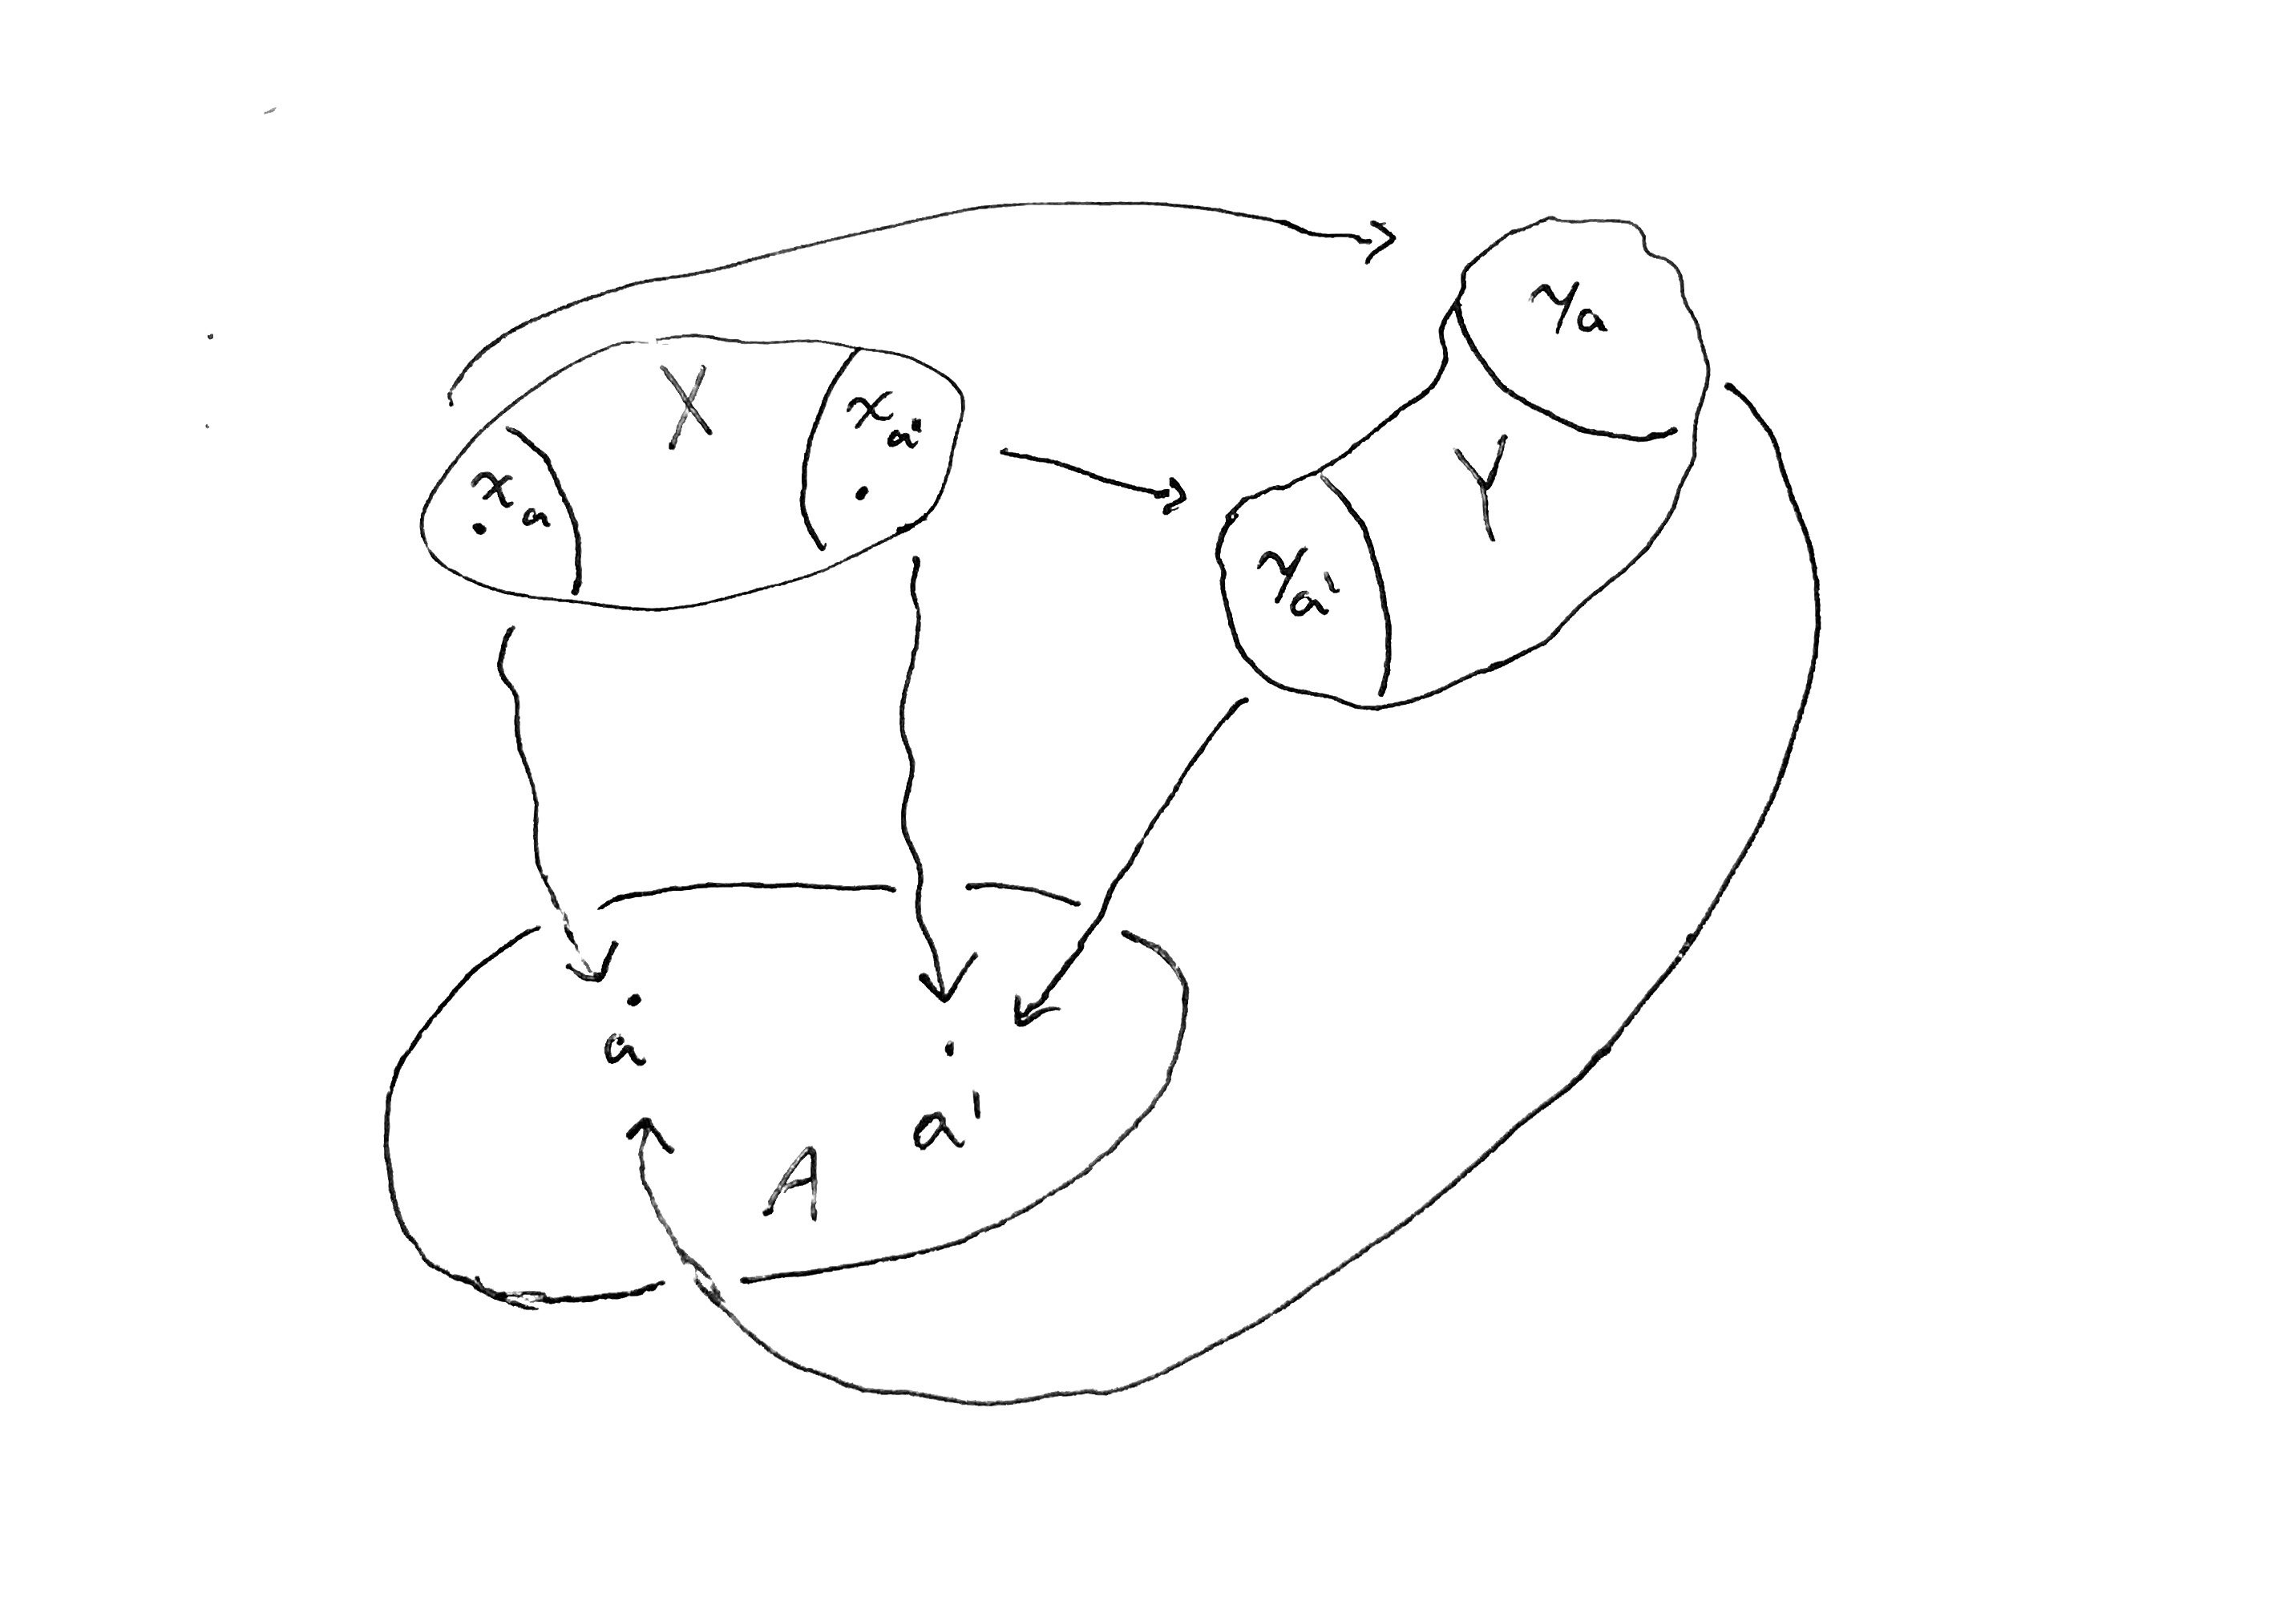
\includegraphics[scale=.1]{Figure1_map_over_A}
%\caption{A map $h$ over $A$.} 
%\end{figure}

Lets look again at what the map $f^*: SET/A \rightarrow SET/B$ induced from $f:B \rightarrow A$ does fiberwise. 

Note that $f^*(\begin{tikzcd}[cramped, sep=small] X \arrow[rd, "p", start anchor={[xshift=-.6ex, yshift= .7ex]},end anchor={[xshift=.7ex, yshift= -.7ex]}]  &  \\  &  A \end{tikzcd})$ is defined by the following pullback diagram:

\setcounter{equation}{0}
\begin{equation}
\begin{tikzcd}
\{(b,x)\in B \times X | fb = px\} \arrow[r] \arrow[d,"f^*p"'] & X \arrow[d,"p"]  \\
B  \arrow[r,"f"'] & A 
\end{tikzcd}
\end{equation}

In the notation of the category $[A^{op},SET]$, we are asking for what $f^*(X_a|a \in A)$ is in $[B^{op},SET]$. To do this we must apply the functor $G_B(\begin{tikzcd}[cramped, sep=small] f^*X \arrow[rd, "f^*p", start anchor={[xshift=-1.5ex, yshift= .7ex]},end anchor={[xshift=.7ex, yshift= -.7ex]}, pos = .4]  &  \\  &  B \end{tikzcd})$.  Thus we must take the preimage $f^*p^{-1}(b)$ for each $b \in B$. For each $b \in B$ the preimage in $\{(b,x)\in B \times X | fb = px\}$ is given by a $b$-indexed subset of $X$ such that for all $x$ in this subset, $px = fb$. Therefore, since we denote the subset of $X$ which maps to $a$ as $X_a$, denote these b-indexed subsets as $X_{fb}$.

\begin{definition}
In $[B^{op}, SET]$, $f^*(X_a|a\in X) = (X_{fb}|b\in B)$. Where $X_{fb} = \{x \in X | fb = px\}$. 
\end{definition}

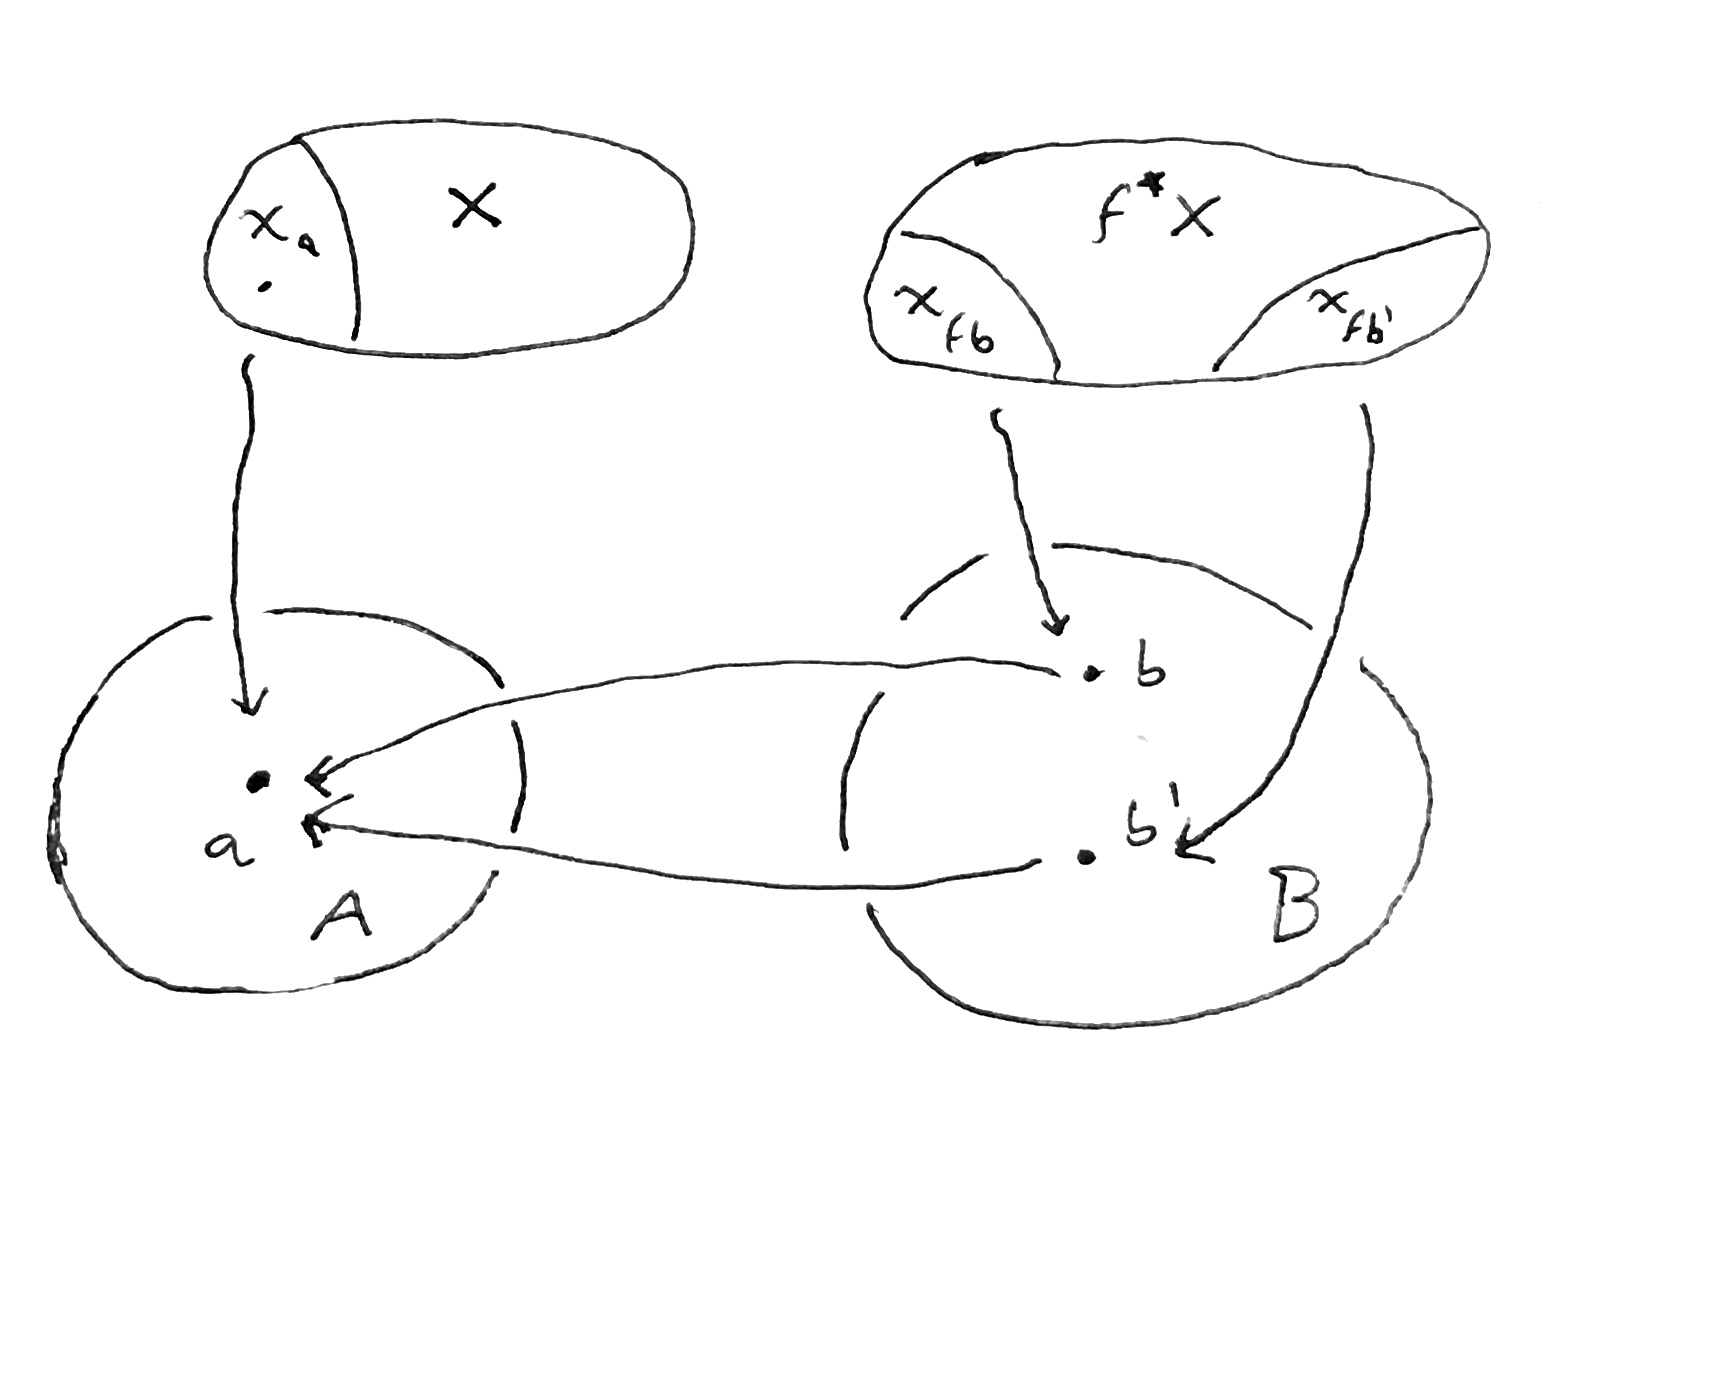
\includegraphics[scale=.15]{Figure2_pullback}

The action of $f^*$ on maps $h$ over $A$ written fiberwise is defined as follows. 

\begin{definition}
In $[B^{op}, SET]$, $$f^*(h_a:X_a \rightarrow Y_a|a \in A) = (h_{fb}:X_{fb} \rightarrow Y_{fb}|b \in B)$$
\end{definition}

This is to say that $f^*$ induces a map of the pullbacks $f^*h:f^*X \rightarrow f^*Y$ and if this map $f^*h$ is going to still be a map over $B$, then it must agree on the fibers. Since the pullback defines the fibers as $X_{fb}$ and $Y_{fb}$, this means that $f^*h$ is a family of maps $X_{fb} \rightarrow Y_{fb}$.\\

Continuing, recall the left adjoint to $f^*$, $\Sigma_f$ defined to be the post composition along $f$ of maps over $B$. Now we examine what it looks like in fiber notation across the equivalence of categories.\\ 

Let $q:Z \rightarrow B$ be a map over $B$, that is, $(Z_b |b \in B)$ where $Z_b = q^{-1}(b)$ and $B_a = f^{-1}(a)$. 

\begin{center}
\begin{tikzcd}
Z \arrow[d, "q"'] \arrow[rd,"\Sigma_fq"]  \\
 B  \arrow[r,"f"'] & A 
\end{tikzcd}
\end{center}

We will need to work out the preimages of each element of $A$ to obtain the representation of $\Sigma_fq$ in $[A^{op},SET]$. Compute, $(\Sigma_fq)^{-1}(a) = (fq)^{-1}(a) = q^{-1}f^{-1}(a) = q^{-1}B_a = \Sigma_{b\in f^{-1}(a)}q^{-1}(b)$ where the final $\Sigma$ is the coproduct. Notice that $q^{-1}B_a = \{q^{-1}(b_1),...,q^{-1}(b_n)\} = \{Z_{b_1},...,Z_{b_n}\} = \Sigma_{b\in f^{-1}(a)}q^{-1}(b)$ is the definition in $SET$ of the coproduct. 

\begin{definition}
In $[A^{op},SET]$ define $\Sigma_f(Z_b|b\in B) = (\Sigma_{b\in B_a}Z_b|a\in A)$.  Note that in the notation of the previous paragraph $Z_b = q^{-1}(b)$ and $B_a = f^{-1}(a)$. \footnote{We are defining the preimage of a set to be the coproduct of the preimages of the points in that set.} 
\end{definition}

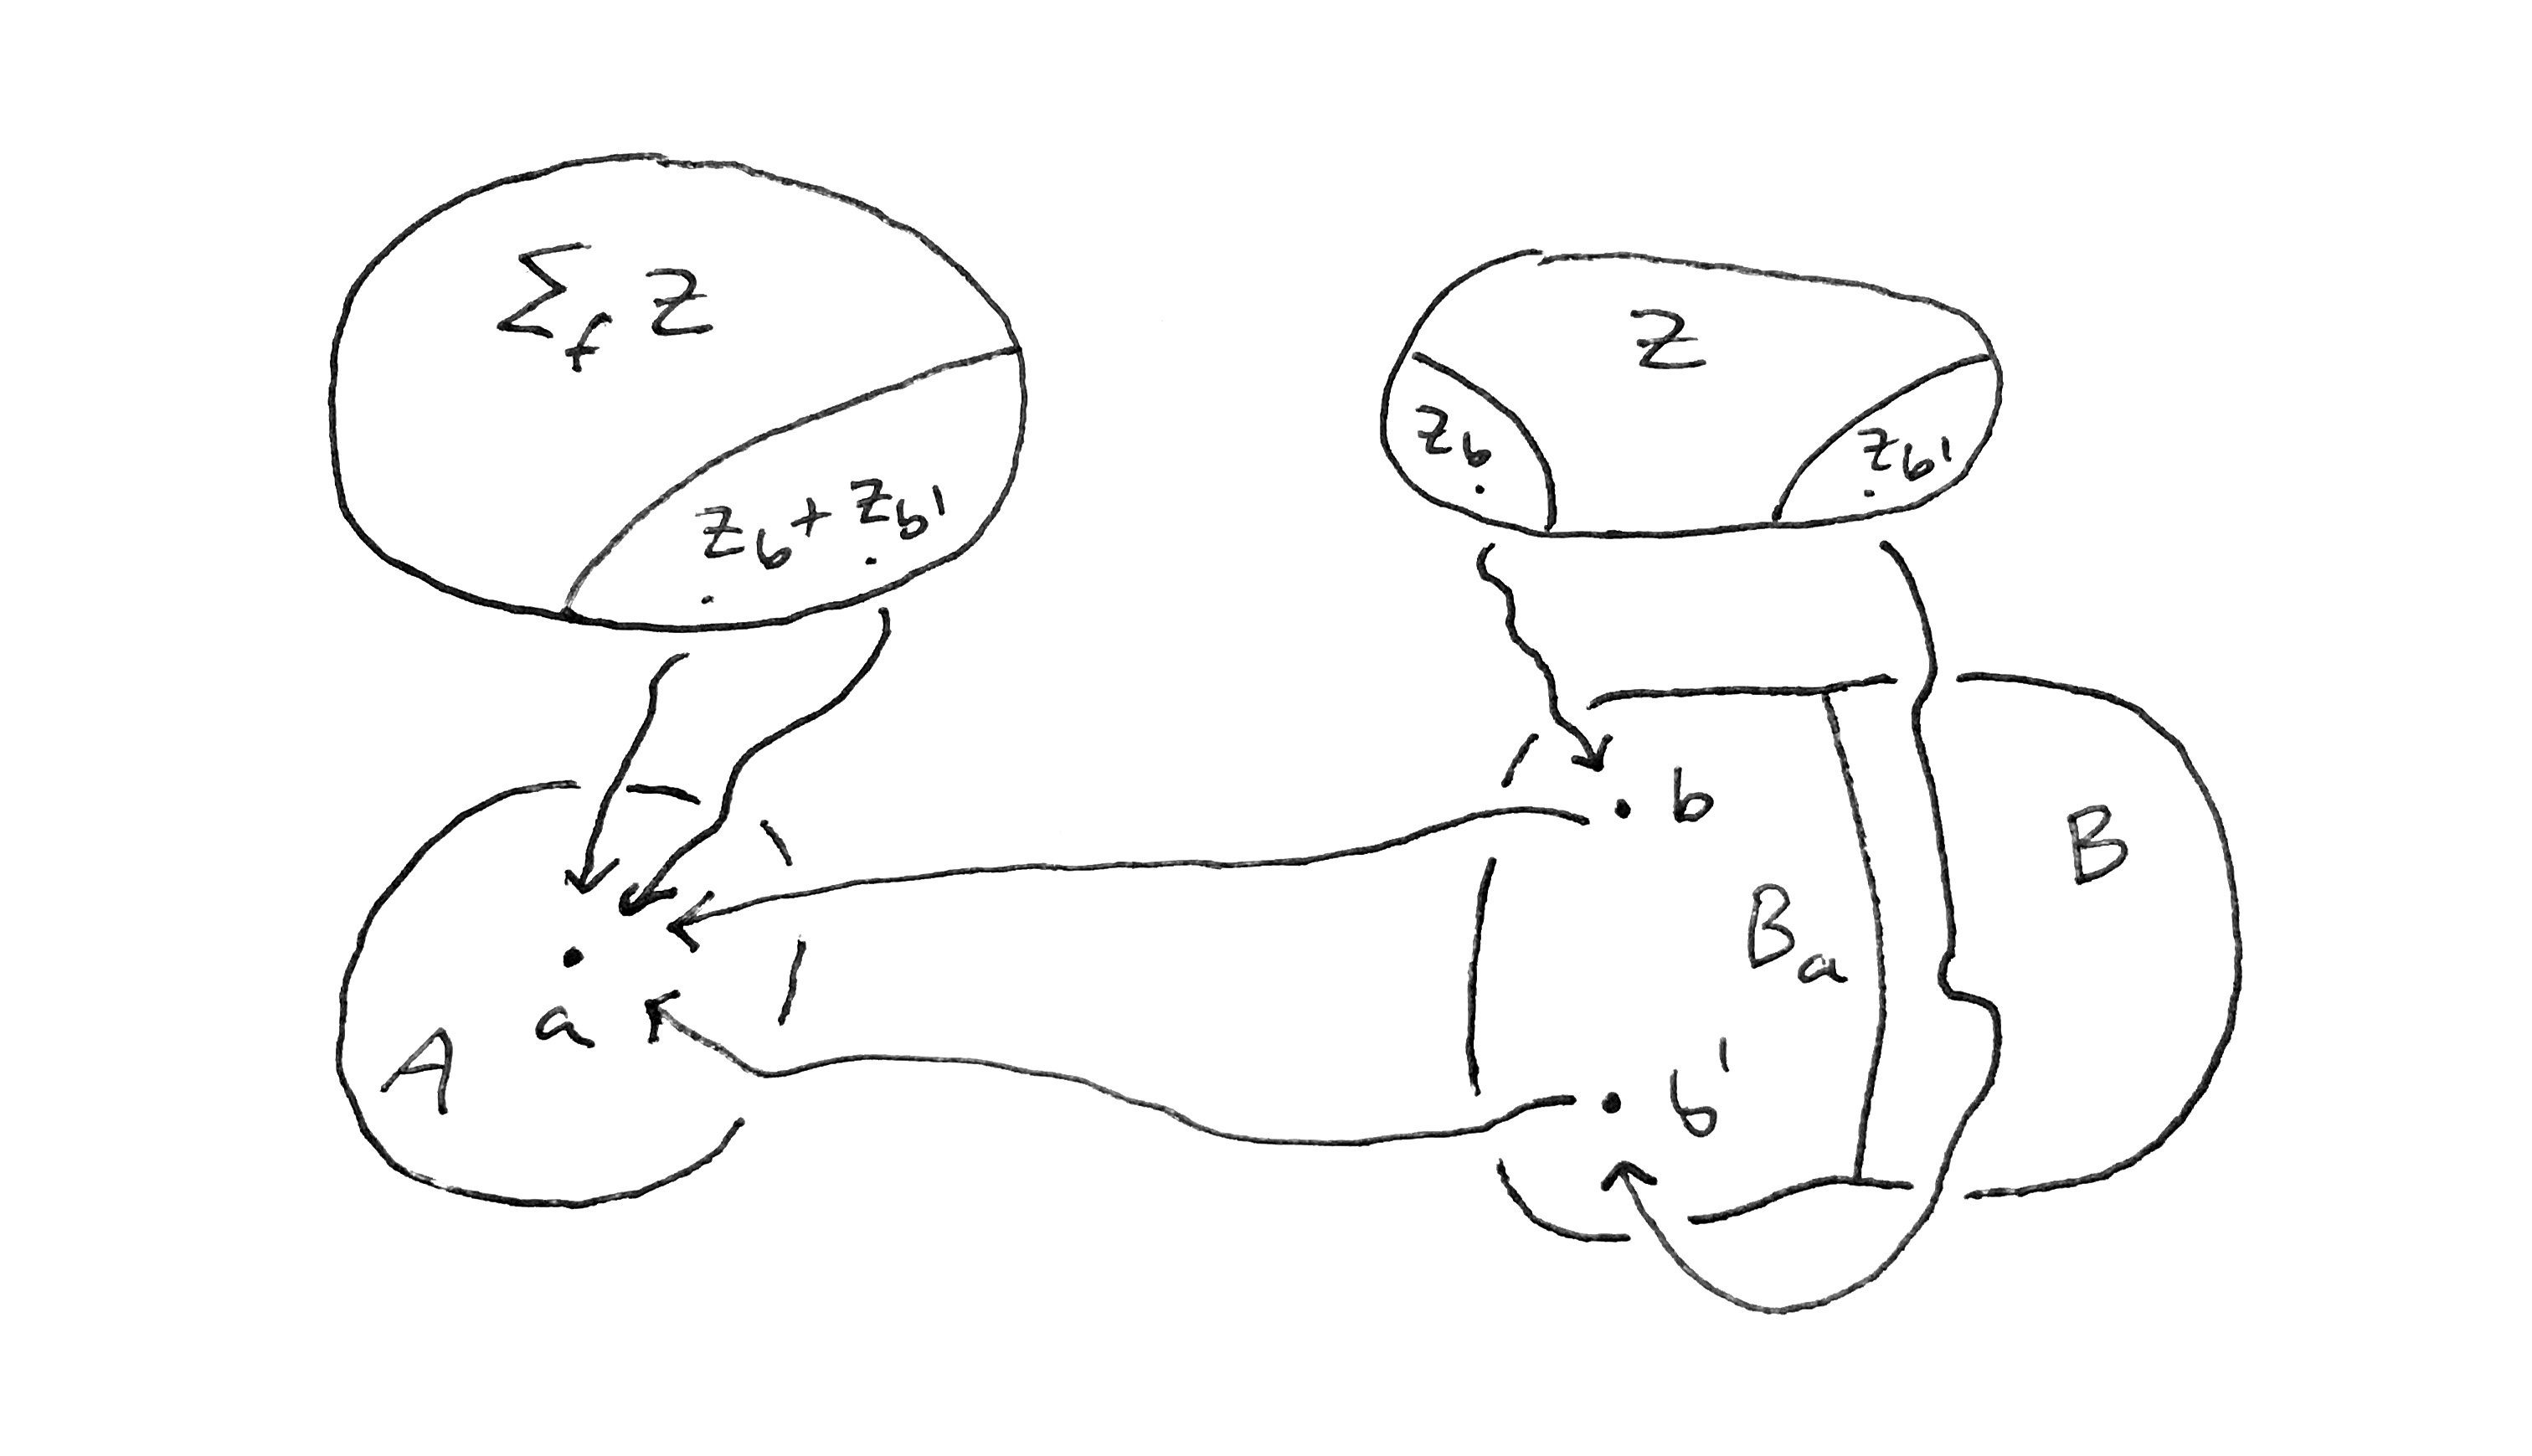
\includegraphics[scale=.1]{Figure3_dependent_sum}

\begin{exercise}
Prove $\Sigma_f(h_b:Z_b \rightarrow Y_b | b \in B) = \Sigma_{b\in B}h_b:\Sigma_{b \in B_a}Z_b \rightarrow \Sigma_{b \in B_a}Y_b$ for all $a \in A$. 
\end{exercise}

\begin{solution}
For each $a \in A$, we need to make a map $\Sigma_{b \in B_a}Z_b \rightarrow \Sigma_{b \in B_a}Y_b$. For each $b \in B_A$ we have a map from $Z_b \rightarrow Y_b \hookrightarrow \Sigma_{b \in B_a}Y_b$, Thus there exists a map $\Sigma_{b\in B}h_b:\Sigma_{b \in B_a}Z_b \rightarrow \Sigma_{b \in B_a}Y_b$ for all $a \in A$. Note that on $\Sigma_{b \in B_a}Z_b$, $\Sigma_{b\in B}h_b = \Sigma_{b\in B_a}h_b$. 
\end{solution}

\begin{exercise}
Find the unit and counit of $\Sigma_f \dashv f^*$.

\begin{center}
\begin{tikzcd}
{[A^{op},SET]} \ar[d, bend left,"","f^*"{name=A, right}]  \\
{[B^{op},SET]} \ar[u, bend left,"","\Sigma_f"{name=B, left}] \ar[from=B, to=A, symbol=\dashv]
\end{tikzcd}
\end{center}

In the following diagram, as above, we do not distinguish between $f^*$ as a map from $SET/A$ to $SET/B$ and it's transpose over the equivalence from solution 2. That is to say, we denote $[f,SET]:[A^{op},SET] \rightarrow [B^{op},SET]$ by $f^*$ also. Similarly, we do not distinguish $\Sigma_f$ from $Lan_{[f,SET]}$, the left adjoint to $[f,SET]$.  
\end{exercise}


\begin{equation}
\begin{tikzcd}
{[A^{op},SET]} \ar[dd, bend left,"F_A",""{name=H, right}] \ar[rr, "f^*"description,""{name=B, right}] & \ & 
{[B^{op},SET]} \ar[ll, bend left,"",""{name=C, right}] \ar[ll, bend right,"\Sigma_f"description,""{name=A, right}]  \ar[dd,bend left, "F_B",""{name=J, left}] \ar[from=A, to=B, symbol=\dashv] \ar[from=B, to=C, symbol=\dashv]  \\
\\
{SET/A} \ar[uu, bend left,"G_A",""{name=G, left}] \ar[rr,"f^*"description,""{name=E, right}]  & \ &
{SET/B} \ar[ll, bend left, "",""{name=F, right}] \ar[ll, bend right, "\Sigma_f"description,""{name=D, right}] \ar[uu,bend left, "G_B",""{name=I, right}]  \ar[from=D, to=E, symbol=\dashv] \ar[from=E, to=F, symbol=\dashv]  \ar[from=G, to=H, symbol=\cong]  \ar[from=I, to=J, symbol=\cong] 
\end{tikzcd}
\end{equation}


\begin{solution}
Combining definition 3 and definition 5 we obtain the data for the unit and counit.\\ 

To obtain the unit we need to find a map $$(Z_b|b \in B) \rightarrow f^*\Sigma_f(Z_b|b \in B)$$ which is natural in B. We compute $$f^*\Sigma_f(Z_b|b\in B) = f^*(\Sigma_{b\in B_a}Z_b|a\in A) = (\Sigma_{b\in B_{fb'}}Z_b|b'\in B)$$

For every $b' \in B$ take every $b \in B_{fb'}$ and form the coproduct of the $Z_b$. Since $b' \in B_{fb'}$ for each $b'$, $Z_b'$ is always a member of the coproduct for that index. Reindexing $(Z_b|b \in B)$, we have for each $(Z_{b'}|b' \in B) \rightarrow (\Sigma_{b\in B_{fb'}}Z_b|b'\in B)$ simply include $Z_{b'} \hookrightarrow \Sigma_{b\in B_{fb'}}Z_b$ because $Z_{b'}$ is one of the terms in the coproduct.\\  

To find the counit of the adjunction, for a given object $(X_a|a\in X)$ over $A$ we need to find a natural map, from $\Sigma_ff^*(X_a|a\in X) \rightarrow (X_a|a\in X)$. We compute, $$\Sigma_ff^*(X_a|a\in X) = \Sigma_f(X_{fb}|b\in B) = (\Sigma_{b\in B_a}X_{fb}|a\in A) =  (\Sigma_{b\in B_a}X_a|a\in A)$$

If $b \in B_a$, then $fb = a$ which gives us the last equality above. Since then for all such $b$ we have $X_{a} \hookrightarrow X_a$, we also have for all $a$, $\Sigma_{b\in B_a}X_{fb} \rightarrow X_a$. Alternatively, $(\Sigma_{b\in B_a}X_a|a\in A) = (B_a\times X_a|a \in A)$. Thus there is a natural map $(\varepsilon_{A_a}:\Sigma_{b\in B_a}X_{a} \rightarrow X_a|a\in X)$ over $A$. This is the counit of the adjunction.\\


\end{solution}

\begin{exercise}
Show that if this adjunction and a terminal object exist then the category $\mathcal{C}$ has products. Define $(-)\times B$ to be the composite map $$\mathcal{C}\xrightarrow[]{\cong} \mathcal{C}/\textbf{1} \xrightarrow[]{\mathcal{C}/B^*} \mathcal{C}/B \xrightarrow[]{\Sigma_k} \mathcal{C}/\textbf{1} \xrightarrow[]{\cong} \mathcal{C}$$
\end{exercise}

\begin{solution}
By examining the above problem closely, we see that this is simply the counit described above in the case where $A = \textbf{1}$ in diagram (1). We have that $$X_{fb} = \{x \in X | px = fb\}$$ but in every case, $px = fb$ because they are both equal to the single element of $\textbf{1}$. Thus $X_{fb} = X$ for every $b$. Similarly, $B_a = B$ because there is again just a single element of $B$. Thus the quantity $(\Sigma_{b\in B_a}X_{fb}|a \in \textbf{1}) = \Sigma_{b \in B}X = X \times B$. 
\end{solution}

{ \ }


\begin{flushleft}
\textbf{The left adjoint $\Pi_f$}
\end{flushleft}

Suppose now we have $f:B \rightarrow A$ in $\mathcal{C}$, an LCC. What is $\Pi_f(\begin{tikzcd}[cramped, sep=small] Z \arrow[rd, "q", start anchor={[xshift=-.6ex, yshift= .7ex]},end anchor={[xshift=.7ex, yshift= -.7ex]}]  &  \\  &  B \end{tikzcd})$? 

Again, moving upward across the equivalence of categories shown in diagram (2), we think of $\begin{tikzcd}[cramped, sep=small] Z \arrow[rd, "q", start anchor={[xshift=-.6ex, yshift= .7ex]},end anchor={[xshift=.7ex, yshift= -.7ex]}]  &  \\  &  B \end{tikzcd}$ as $(Z_b|b \in B)$. The adjunction we are examining takes the form 

$$
\mathcal{C}/A(
\begin{tikzcd}[cramped, sep=small] X \arrow[rd, "p", start anchor={[xshift=-.6ex, yshift= .7ex]},end anchor={[xshift=.7ex, yshift= -.7ex]}]  &  \\  &  A \end{tikzcd}
,\Pi_f(\begin{tikzcd}[cramped, sep=small] Z \arrow[rd, "q", start anchor={[xshift=-.6ex, yshift= .7ex]},end anchor={[xshift=.7ex, yshift= -.7ex]}]  &  \\  &  B \end{tikzcd}))
\cong
\mathcal{C}/B(f^*(
\begin{tikzcd}[cramped, sep=small] X \arrow[rd, "p", start anchor={[xshift=-.6ex, yshift= .7ex]},end anchor={[xshift=.7ex, yshift= -.7ex]}]  &  \\  &  A \end{tikzcd})
,\begin{tikzcd}[cramped, sep=small] Z \arrow[rd, "q", start anchor={[xshift=-.6ex, yshift= .7ex]},end anchor={[xshift=.7ex, yshift= -.7ex]}]  &  \\  &  B \end{tikzcd})
$$

Using the right side of the adjunction we will investigate what form $\Pi_f$ will take. Moving across the equivalence, $f^*(
\begin{tikzcd}[cramped, sep=small] X \arrow[rd, "p", start anchor={[xshift=-.6ex, yshift= .7ex]},end anchor={[xshift=.7ex, yshift= -.7ex]}]  &  \\  &  A \end{tikzcd}) = f^*(X_a|a\in A) = (X_{fb}|b \in B)$. 

Maps $(h_b:X_{fb} \rightarrow Z_b|b \in B)$ are maps $(\overline{h}_a:X_a\rightarrow \Pi_f(Z)_a|a \in A)$.\\

\begin{example}

Let $A = \{a_1,a_2\}$, $B = \{b_1,b_2,b_3\}$, $X = \{x_1,x_2,x_3,x_4\}$, and $Z = \{z_1,z_2,z_3\}$. Define $p:X\rightarrow A$ by $p(x_1) = p(x_2) = a_1$ and $p(x_3) = p(x_4) = a_2$.  Define $q:Z\rightarrow B$ by $q(z_1) = b_1$, $q(z_2) = b_2$, and $q(z_3) = b_3$. \\

In the context of this example, one can check that $$f^*X = \{(x_1,b_1),(x_1,b_2),(x_2,b_1),(x_2,b_2),(x_3,b_3),(x_4,b_3)\}$$  alternatively, $$f^*X = \{X_{fb_1},X_{fb_2},X_{fb_3}\}$$ where $X_{fb1} = \{x_1,x_2\}$. Thus we can write $$f^*X = \{\{x_1,x_2\}_{b_1},\{x_1,x_2\}_{b_2},\{x_3,x_4\}_{b_3}\}$$\\ 

An example of a map $h$ over $B$, $(h_b:X_{fb} \rightarrow Z_b|b \in B)$ would be a collection of maps $$h_{b_1}:\{x_1,x_2\}_{b_1} \rightarrow \{z_1\}$$
$$h_{b_2}:\{x_1,x_2\}_{b_2} \rightarrow \{z_2\}$$
$$h_{b_3}:\{x_3,x_4\}_{b_3} \rightarrow \{z_3\}$$
Such maps over $B$ must correspond to maps $(\overline{h}_a:X_a\rightarrow \Pi_f(Z)_a|a \in A)$. 
$$\overline{h}_{a_1}:\{x_1,x_2\}\rightarrow \Pi_f(Z)_{a_1}$$
$$\overline{h}_{a_2}:\{x_3,x_4\}\rightarrow \Pi_f(Z)_{a_2}$$
If there exist maps $h_{b_1}$ and $h_{b_2}$ out of $X_{fb_1}$ and $X_{fb_2}$ which are copies, then there exists a map from $\{x_1,x_2\} \rightarrow {a_1}\times{a_2}$. 
\end{example}

\begin{definition}
Define $\Pi_f(\begin{tikzcd}[cramped, sep=small] Z \arrow[rd, "q", start anchor={[xshift=-.6ex, yshift= .7ex]},end anchor={[xshift=.7ex, yshift= -.7ex]}]  &  \\  &  B \end{tikzcd}) = (\Pi_{b \in B_a}Z_b|a \in A)$. 
\end{definition}

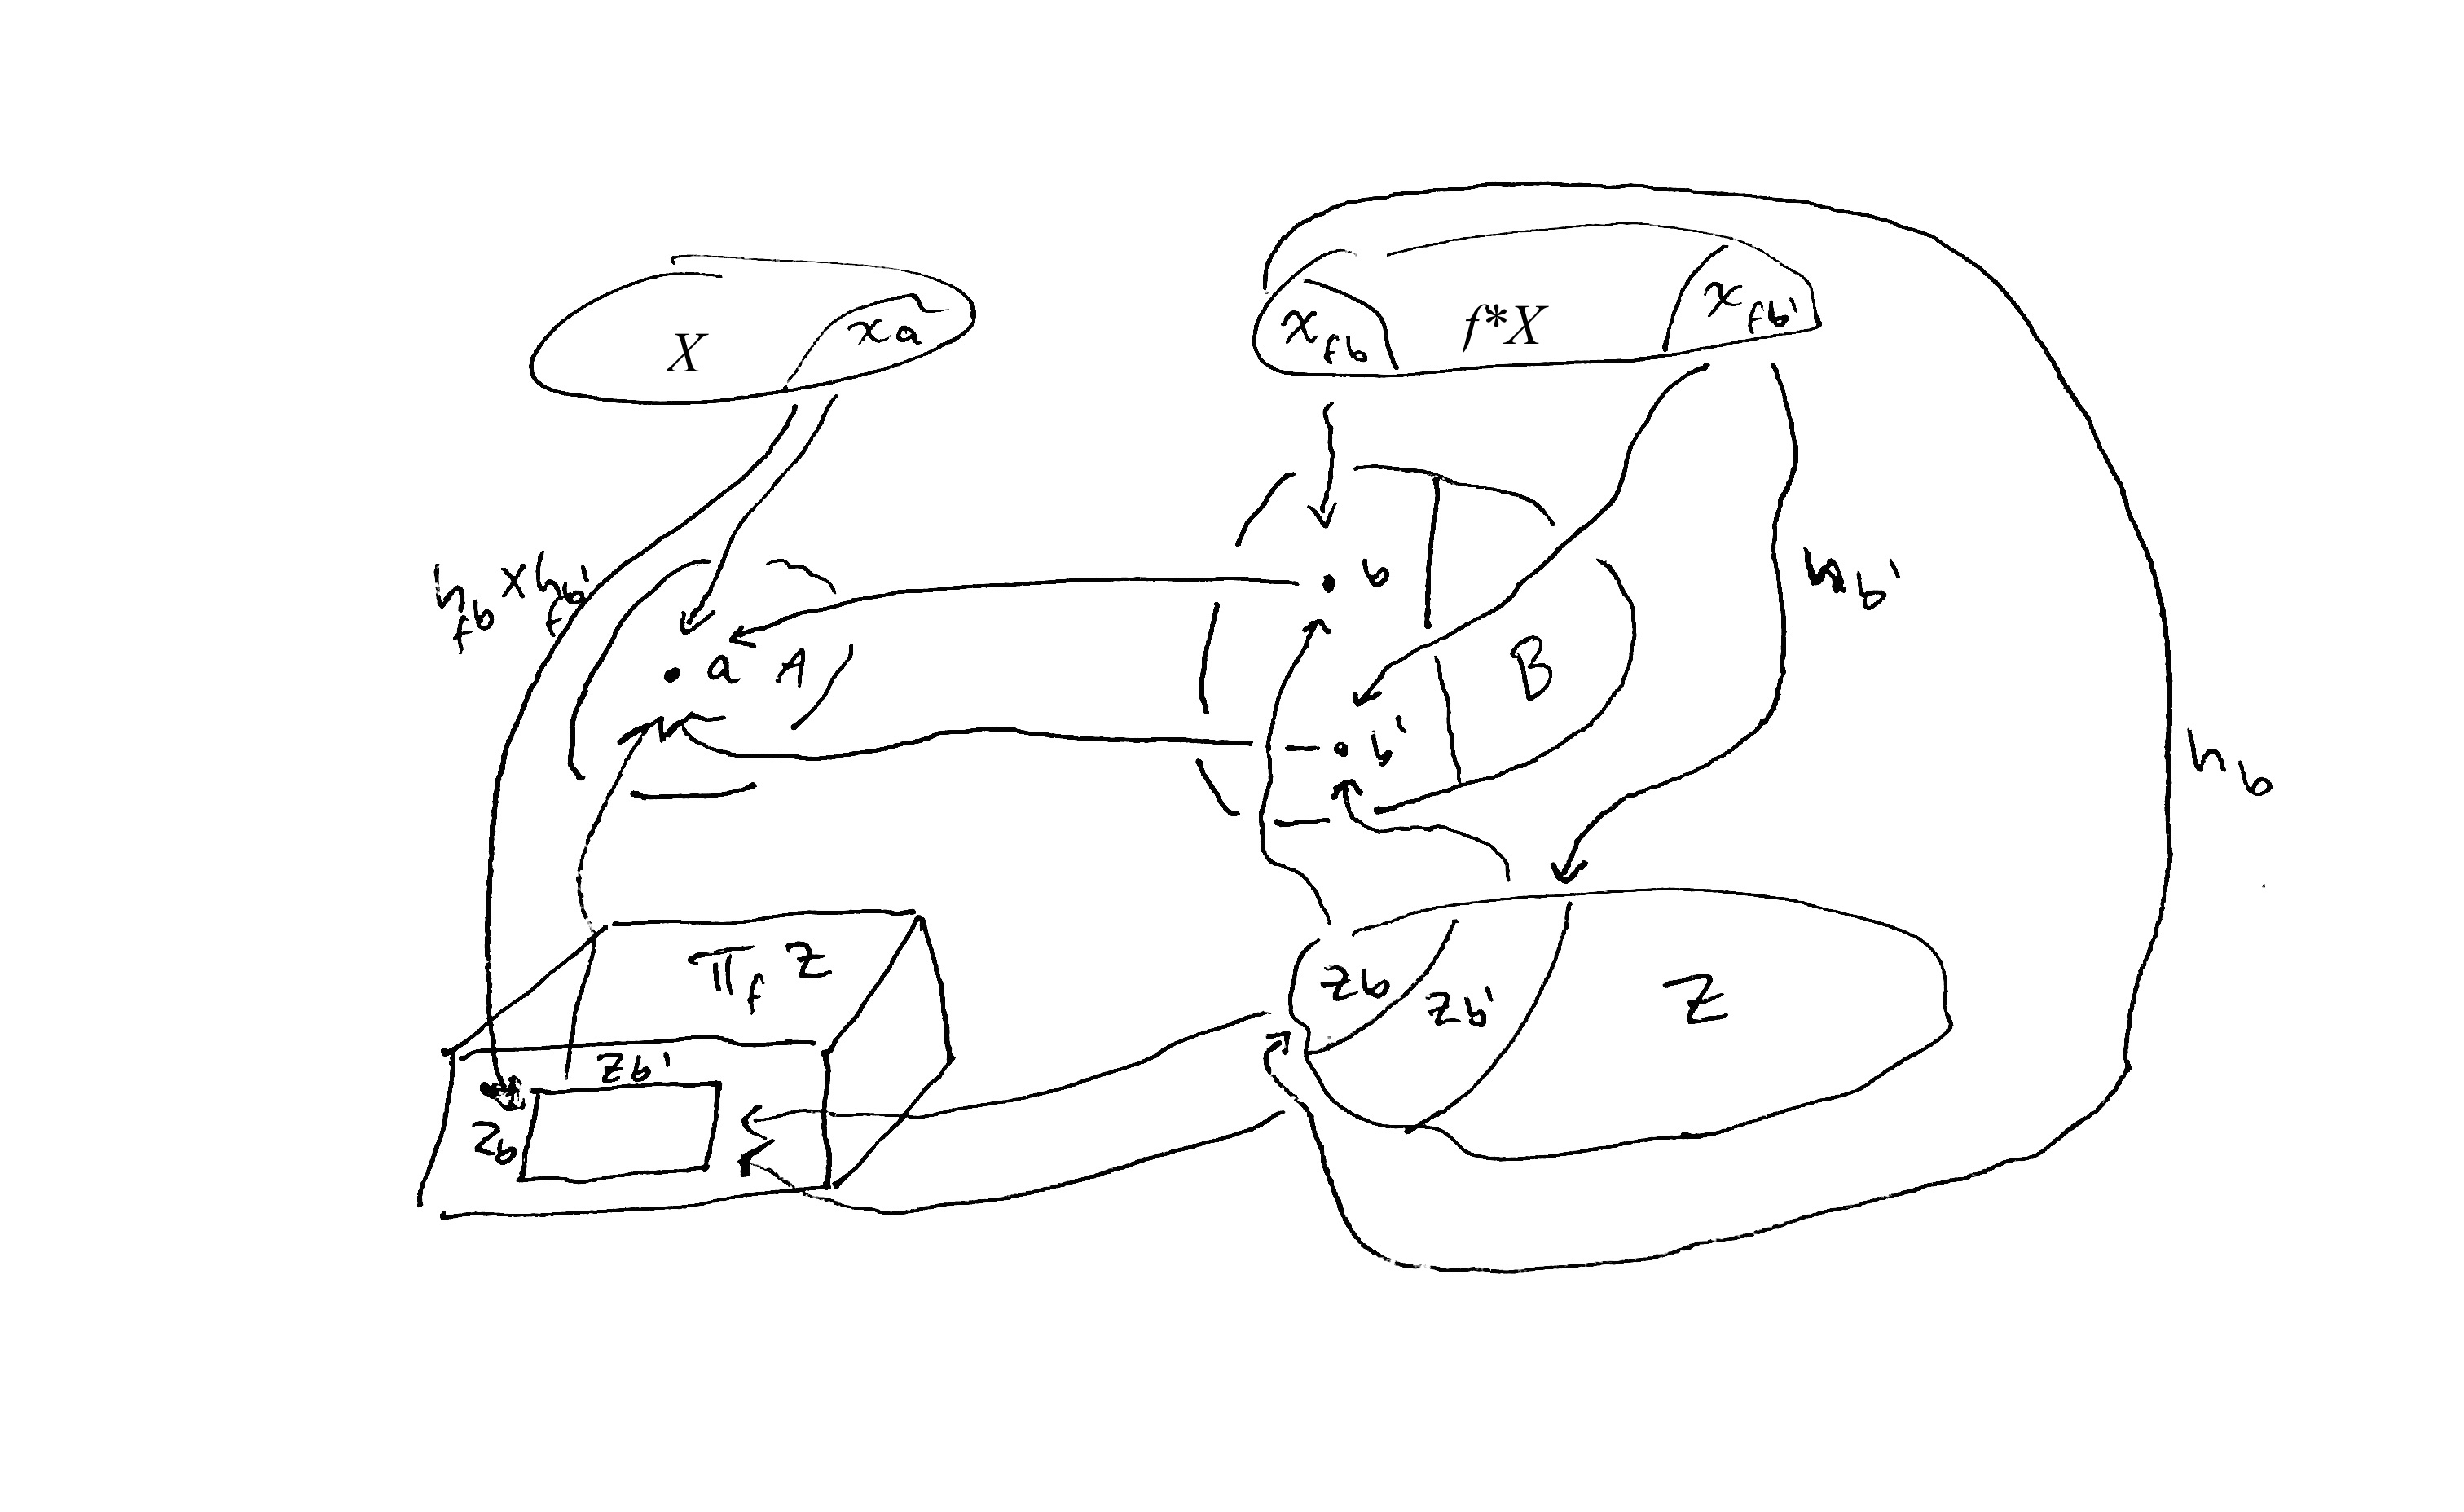
\includegraphics[scale=.12]{Figure4_dependent_product}
\flushleft
How shall we read $\Pi_{b\in B_a}Z_b$? We can read it as either, 

\begin{enumerate}
\item products of sets
\item sequences of values indexed by $B_a$
\item functions $f:B_a\rightarrow (Z_b|b \in B)$
\end{enumerate}

\begin{example}
In the case $B_a = B$ for every $a \in A$, and $Z_b = Z$ for all $b \in B$ we have  $\Pi_f(\begin{tikzcd}[cramped, sep=small] Z \arrow[rd, "q", start anchor={[xshift=-.6ex, yshift= .7ex]},end anchor={[xshift=.7ex, yshift= -.7ex]}]  &  \\  &  B \end{tikzcd}) = (\Pi_{b \in B_a}Z_b|a \in A) = (\Pi_{b \in B}Z|a \in A) = (Z^B|a \in A)$.
\end{example}

\begin{center}
\begin{tikzcd}
{[B^{op},SET]} \ar[d, bend left,"","\Pi_f"{name=A, right}]  \\
{[A^{op},SET]} \ar[u, bend left,"","f^*"{name=B, left}] \ar[from=B, to=A, symbol=\dashv]
\end{tikzcd}
\end{center}

What is the unit and counit of the adjunction $f^* \dashv \Pi_f$? The unit is going to be an $A$ indexed family of maps: 
$$\eta_{(X_a|a \in A)}:(X_a|a \in A)\rightarrow\Pi_ff^*(X_a|a \in A) = \Pi_f(X_{fb}|b \in B) = (\Pi_{b\in B_a}X_{fb}|a\in A)$$ which can be written more succinctly as $$(\eta_a:X_a\rightarrow \Pi_{b\in B_a}X_{fb}|a\in A)$$ because $b \in B_a$ ensures that $fb = a$ we may write the definition as follows

\begin{definition}
We define the unit of the adjunction $f^* \dashv \Pi_f$ to be the $A$ indexed family of maps $(\eta_a:X_a\rightarrow \Pi_{b\in B_a}X_{a}|a\in A)$ where these maps are given in multiple contexts as either 
\begin{enumerate}
\item the diagonal (product of sets)
\item constant sequence (sequences of values)
\item constant function (functions $f:B_a\rightarrow (X_a|a \in A)$)
\end{enumerate}
\end{definition}

\begin{example}
In order to find the counit we compute the following

$$f^*\Pi_f(Z_b |b \in B) = f^*(\Pi_{b'\in B_a}Z_{b'}|a \in A) = (\Pi_{b' \in B_{fb}}Z_{b'}|b \in B)$$

A map from $f^*\Pi_f(Z_b |b \in B)$ to $(Z_b |b \in B)$ is given by the $b^{\text{th}}$ projection, the $b^{\text{th}}$ term or the evaluation of the choice function at $b$. 
\end{example}

\begin{definition}
We define the counit of the adjunction $f^* \dashv \Pi_f$ to be the $B$ indexed family of maps $(\varepsilon_b:\Pi_{b' \in B_{fb}}Z_{b'}\rightarrow Z_b|b \in B)$ where these maps are given in multiple contexts as either 
\begin{enumerate}
\item $b^{\text{th}}$ the projection (product of sets)
\item $b^{\text{th}}$ term (sequences of values)
\item evaluation at $b$ (functions $f:B_{fb}\rightarrow (Z_b|b \in B)$)
\end{enumerate}
\end{definition}

\begin{exercise}
What are the traingle equalities saying?\\ 
\vspace{5mm} %5mm vertical space
Applying $f^*$ to the following diagram $(\eta_a:X_a \rightarrow \Pi_{b \in B_a}X_{fb}|a \in A)$, we obtain, $$(f^*\eta_b:X_{fb} \rightarrow \Pi_{b'\in B_{fb}}X_{fb'}|b \in B)$$ Applying $\varepsilon_{f^*X}$ we obtain, $$((id_{f^*})_b = (\varepsilon_{f^*X} \circ f^* \circ \eta_{f^*X})_b:X_{fb} \rightarrow \Pi_{b'\in B_{fb}}X_{fb'} \rightarrow X_{fb}|b \in B)$$

Roughly this is saying, for each $b$, the inclusion of $X_{fb}$ into a $B_{fb}$ indexed power of $X_{fb}$ followed by projection onto a single copy of $X_{fb}$ again is the identity.\\
\vspace{5mm} %5mm vertical space
To find the second triangle equality, we apply the unit $\eta$ at $\Pi_f(Z_b|b\in b) = (\Pi_{b' \in B_a}Z_{b'}|a \in A)$ to obtain $$(\eta_a:\Pi_{b \in B_a}Z_b \rightarrow \Pi_{b \in B_a}(\Pi_{b' \in B_{fb}}Z_{b'})|a \in A)$$
Appling $\Pi_f$ to the counit $(\varepsilon_b:\Pi_{b' \in B_{fb}}Z_{b'}\rightarrow Z_b|b \in B)$ we obtain a map $(\Pi_f \circ \varepsilon_a:\Pi_{b\in B_a}{\Pi_{b' \in B_{fb}}Z_{b'}}\rightarrow \Pi_{b \in B_a}Z_b|a \in A)$. The composition of these maps modulo reindexing yeilds a map equal to the identity at $\Pi_f(Z)$ $$((id_{\Pi_f(Z)})_a = (\Pi_f \ \circ \ \varepsilon \ \circ \ \eta_{\Pi_f(Z)})_a:\Pi_{b \in B_a}Z_b \rightarrow \Pi_{b \in B_a}(\Pi_{b' \in B_{fb}}Z_{b'}) \rightarrow \Pi_{b \in B_a}Z_{b}|a \in A)$$

We can interpret this as the statement, for each $a \in A$, the product of the $Z_b$ where $b \in B_a$ can be included into the $(\Pi_{b\in B_a}Z_b)^{B_a}$ as the diagonal map. Then for each $b' \in B_a$, project the $b'$th term of $(\Pi_{b\in B_a}Z_b)^{B_a}$ onto $Z_{b'}$. Thus we obtain a map into $\Pi_{b' \in B_a}Z_b'$. 
\end{exercise}

\begin{lemma}
Let $\mathcal{C}$ be an LCC. Let  $B \xrightarrow[]{f} A$.  Then in $\mathcal{C}/A$, the composite
$$\mathcal{C}/A\xrightarrow[]{f^*} \mathcal{C}/B \xrightarrow[]{\Sigma_f} \mathcal{C}/A$$
is the product $(-)\times(\begin{tikzcd}[cramped, sep=small] B \arrow[rd, "f", start anchor={[xshift=-.6ex, yshift= .7ex]},end anchor={[xshift=.7ex, yshift= -.7ex]}]  &  \\  &  A \end{tikzcd}).$
\end{lemma}

\begin{proof}{internal}
$$\Sigma_ff^*(X_a|a \in A) = \Sigma_f(X_{fb}|b \in B) = (\Sigma_{b\in B_a} X_{fb}|a \in A) =$$
$$(\Sigma_{b\in B_a}X_{a}|a \in A) = (X_a\times B_a|a\in A)$$

Given an object $(Y_a|a\in A)$ and maps $(h_a:Y_a\rightarrow B_a|a\in A)$ and $(k_a:Y_a\rightarrow X_a|a\in A)$ we have a unique map $(l_a:Y_a \rightarrow X_a\times B_a|a \in A)$ where $(l_a = h_a\times k_a|a\in A)$. The obvious projections exist.  
\end{proof}

\begin{proof}{external}

Using the diagram below, let $h$ and $k$ be maps over $A$. Since $f\circ k = i = p \circ h$, we have  $f\circ k = p \circ h$ so we obtain a map $l$ from $Y$ to $f^*X$ because it is a pullback. Since the entire diagram commutes, $f^*X = \Sigma_ff^*X$ is the product with projections $\varepsilon_X$ and $f^*p$. 
\begin{center}
\begin{tikzcd}
Y
\arrow[drrr, bend left, "h"]
\arrow[dddr, bend right, "k"']
\arrow[dddrrr, bend right, "i"',pos = .3, end anchor={[xshift=-.9ex, yshift= .7ex]}]
\arrow[dr, "l"] & & \\
& \Sigma_ff^*X = f^*X \arrow[rr, "\varepsilon_X"]  \arrow[dd, line width=7pt,draw=white,dash] \arrow[dd, "f^*p", pos = .4] \arrow[ddrr, "\Sigma_ff^*p", pos = .4]
& &  X \arrow[dd, "p"] \\
& & \\
& B \arrow[rr, "f"']
& &  A
\end{tikzcd}
\end{center}
\end{proof}

\begin{lemma}
If $\mathcal{C}$ is LCC then $\mathcal{C}/A$ has product $(-)\times(\begin{tikzcd}[cramped, sep=small] B \arrow[rd, "f", start anchor={[xshift=-.6ex, yshift= .7ex]},end anchor={[xshift=.7ex, yshift= -.7ex]}]  &  \\  &  A \end{tikzcd})$ has a right adjoint. 
\end{lemma}

\begin{proof}
We may compose the following adjunctions
\begin{center}
\begin{tikzcd}
{\mathcal{C}/A} \ar[r, bend left,"","f^*"{name=A}] & {\mathcal{C}/B} \ar[l, bend left,"","\Pi_f"{name=B}] \ar[r, bend left,"","\Sigma_f"{name=C}] & {\mathcal{C}/A} \ar[l, bend left,"","f^*"{name=D}] \ar[from=A, to=B, symbol=\dashv]  \ar[from=C, to=D, symbol=\dashv] 
\end{tikzcd}
\end{center}
to obtain 
\begin{center}
\begin{tikzcd}
{\mathcal{C}/A} \ar[r, bend left,"","{\Sigma_f \circ f^*}"{name=A}] & {\mathcal{C}/A} \ar[l, bend left,"","\Pi_f\circ f^*"{name=B}] \ar[from=A, to=B, symbol=\dashv] 
\end{tikzcd}
\end{center}

However, by lemma 1, $\Sigma_f \circ f^* = (-)\times(\begin{tikzcd}[cramped, sep=small] B \arrow[rd, "f", start anchor={[xshift=-.6ex, yshift= .7ex]},end anchor={[xshift=.7ex, yshift= -.7ex]}]  &  \\  &  A \end{tikzcd}).$ We compute the value of the right adjoint, $$\Pi_ff^*(Y_a|a\in A) = \Pi_f(Y_{fb}|b \in B)$$ 
$$ = (\Pi_{b\in B_a}Y_{fb}|a\in A) = (\Pi_{b\in B_a}Y_{a}|a\in A) = (Y_a^{B_a}|a \in A)$$ and see that indeed it is the fiberwise exponential. 

\begin{center}
\begin{tikzcd}
{\mathcal{C}/A} \ar[dd, bend left,"","(-)^{B \xrightarrow[]{f} A}"{name=B}] \\
\\
{\mathcal{C}/A} \ar[uu, bend left,"","{(-)\times (B \xrightarrow[]{f} A)}"{name=A}]  
\ar[from=A, to=B, symbol=\dashv] 
\end{tikzcd}
\end{center}

\end{proof}

This completes the proof of the following theorem. 

\begin{theorem}
If $\mathcal{C}$ is $LCC$ then $\mathcal{C}/A$ is $CC$ for any object $A$ of $\mathcal{C}$.
\end{theorem}

\end{document}